% Design
\section{Design}

\subsection{Package-Struktur}

Die Package-Struktur wird vom Sencha Touch 2 Framework vorgegeben. Sie entspricht grundsätzlich dem MVC-Layout.
Speziell daran ist aber das Konzept der \emph{Stores}, welche einen beliebigen Datenspeicher abstrahieren.
Stores sind an ein \emph{Model} gebunden, welches die Struktur der gespeicherten Daten vorgibt.

Zusätzlich sind sie über einen \emph{Proxy} mit der Datenquelle verbunden.
Dabei kann es sich beispielsweise um einen \gls{REST}-Webservice handeln oder den \gls{Local Storage} des Browsers.

In Abbildung \ref{kort-packages} ist die Package-Struktur von \textsc{Kort} dargestellt.

\begin{figure}[H]
	\centering
	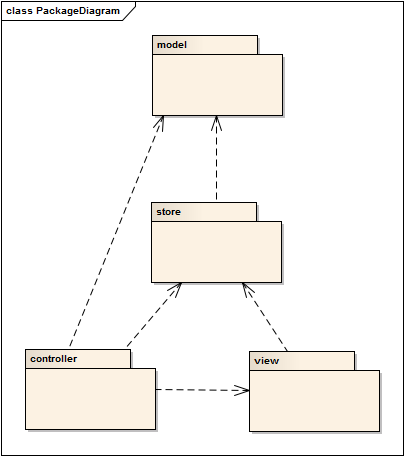
\includegraphics[scale=0.7]{images/uml/kort-packagediagram}
	\caption{kort - Package-Struktur}
	\label{kort-packages}
\end{figure}

\subsection{Controller-Package}

Die App wurde so gestaltet, dass jede Hauptansicht seinen eigenen Controller besitzt.
Dieser ist für die Steuerung der Benutzeroberfläche zuständig.

Die Controller lassen sich wiederum in drei Klasen einteilen.
Zum einen gibt es Controller für die einzelnen Tabs der Applikation (siehe Abbildung \ref{kort-controller} $\rightarrow$ \emph{main tab controllers}).
Zusätzlich haben einige Tabs eine Detailansicht, welche ebenfalls von einem eigenen Controller gesteuert wird (siehe Abbildung \ref{kort-controller} $\rightarrow$ \emph{detail controllers}).
Zuletzt gibt es noch eigenständige Controller für die Overlay-Komponenten, welche die gesamte Oberfläche der App verdecken (siehe Abbildung \ref{kort-controller} $\rightarrow$ \emph{overlay controllers}).

\begin{figure}[H]
	\centering
	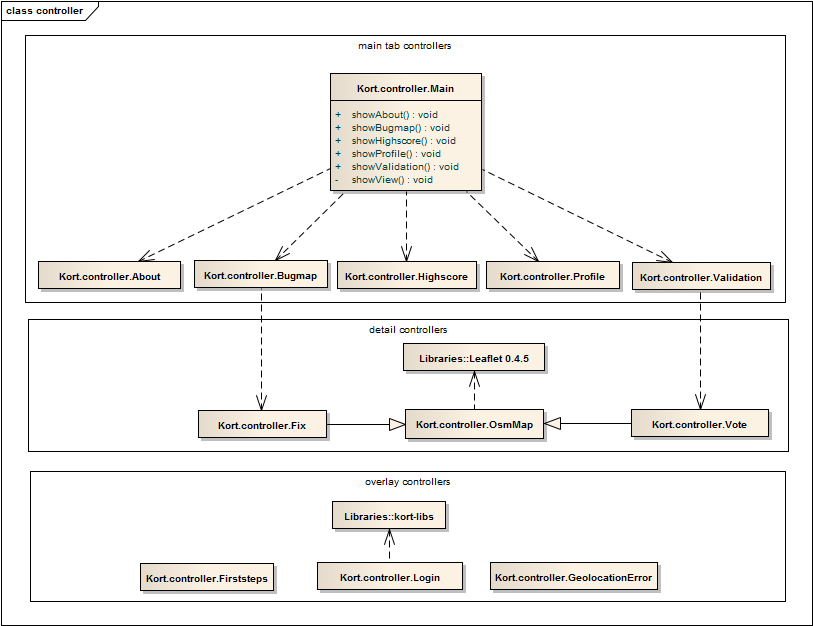
\includegraphics[width=\textwidth]{images/uml/kort-classdiagram-controller}
	\caption{kort - Controller}
	\label{kort-controller}
\end{figure}

\subsection{Store- und Model-Package}

